\chapter{Image Filtering}

\section{Linear Shift-Invariant Filters}

\subsection{Definition}

A filter transforms one signal into another. Filters are used to describe image formation (lens burring, sensor noise, etc.), as well as to implement operations on images (edge detection, noise reduction, etc.).

\begin{figure}[ht!]
    \centering
    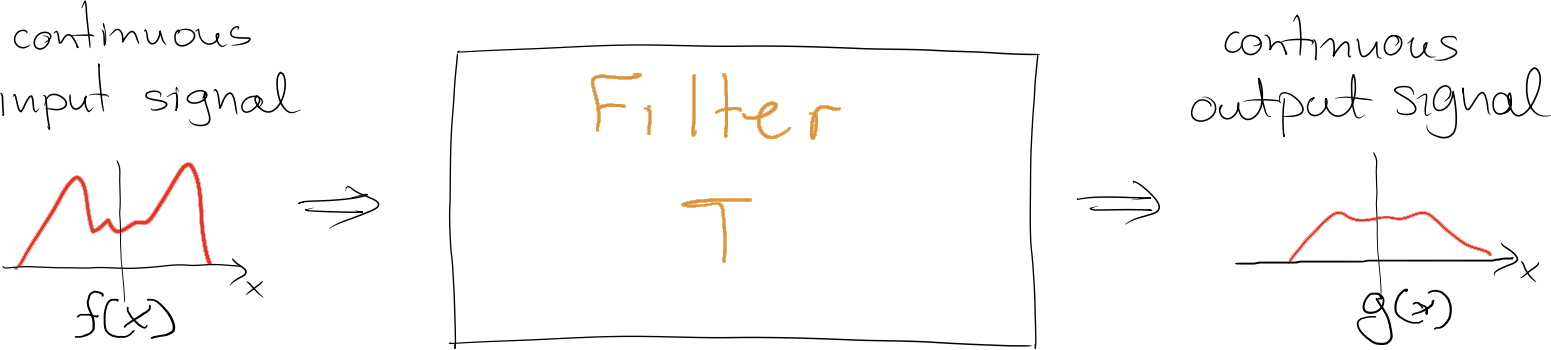
\includegraphics[width=0.75\linewidth]{figures/filter.png}
\end{figure}

\begin{definition}[Linear Transformation]\index{Linear Transformation}\label{def:linear-transformation}
    A transformation $T$ is \term{linear} if and only if it satisfies \[
        T[a_1 f_1(x) + a_2 f_2(x)] = a_1 T[f_1(x)] + a_2 T[f_2(x)]
    \] for any $a_1, a_2 \in \mathbb{R}$ and continuous functions $f_1, f_2$. 
\end{definition}

Every linear transformation between functions $f, g$ can be expressed as an integral of the form \[
    g(x) = \int_{-\infty}^{\infty} h(x, \tau) f(\tau) \, d\tau,
\] where the $h(x, \tau)$ is the contribution of position $\tau$ of the input to position $x$ of the output.

% TODO: Add a figure to illustrate shift-invariance

\begin{definition}[Shift-Invariant Filter]\index{Shift-Invariant Filter}\label{def:shift-invariant-filter}
    A filter $h(x, \tau)$ is \term{shift-invariant} if and only if shifted inputs produce identical but shifted outputs. 
\end{definition}

% TODO: Graph of the two functions

Imagine we have the shifted input \[
    f'(x') = f(x - x_0)
\] and the shifted output \[
    g'(x') = g(x - x_0).
\] The \term{shift invariance property} states that \[
    T[f(x - x_0)] = g(x - x_0)
\]

\subsection{The Impulse Function}